%%
%% This is file `sample-authordraft.tex',
%% generated with the docstrip utility.
%%
%% The original source files were:
%%
%% samples.dtx  (with options: `authordraft')
%% 
%% IMPORTANT NOTICE:
%% 
%% For the copyright see the source file.
%% 
%% Any modified versions of this file must be renamed
%% with new filenames distinct from sample-authordraft.tex.
%% 
%% For distribution of the original source see the terms
%% for copying and modification in the file samples.dtx.
%% 
%% This generated file may be distributed as long as the
%% original source files, as listed above, are part of the
%% same distribution. (The sources need not necessarily be
%% in the same archive or directory.)
%%
%% Commands for TeXCount
%TC:macro \cite [option:text,text]
%TC:macro \citep [option:text,text]
%TC:macro \citet [option:text,text]
%TC:envir table 0 1
%TC:envir table* 0 1
%TC:envir tabular [ignore] word
%TC:envir displaymath 0 word
%TC:envir math 0 word
%TC:envir comment 0 0
%%
%%
%% The first command in your LaTeX source must be the \documentclass command.
\documentclass[sigconf,authordraft]{acmart}
%% NOTE that a single column version may required for 
%% submission and peer review. This can be done by changing
%% the \doucmentclass[...]{acmart} in this template to 
%% \documentclass[manuscript,screen]{acmart}
%% 
%% To ensure 100% compatibility, please check the white list of
%% approved LaTeX packages to be used with the Master Article Template at
%% https://www.acm.org/publications/taps/whitelist-of-latex-packages 
%% before creating your document. The white list page provides 
%% information on how to submit additional LaTeX packages for 
%% review and adoption.
%% Fonts used in the template cannot be substituted; margin 
%% adjustments are not allowed.

%%
%% \BibTeX command to typeset BibTeX logo in the docs
%\AtBeginDocument{%
%  \providecommand\BibTeX{{%
%    \normalfont B\kern-0.5em{\scshape i\kern-0.25em b}\kern-0.8em\TeX}}}

%% Rights management information.  This information is sent to you
%% when you complete the rights form.  These commands have SAMPLE
%% values in them; it is your responsibility as an author to replace
%% the commands and values with those provided to you when you
%% complete the rights form.
\setcopyright{acmcopyright}
\copyrightyear{2023}
\acmYear{2023}
\acmDOI{XXXXXXX.XXXXXXX}

%% These commands are for a PROCEEDINGS abstract or paper.
%\acmConference[Conference acronym 'XX]{Make sure to enter the correct
%  conference title from your rights confirmation emai}{June 03--05,
%  2018}{Woodstock, NY}
%
%  Uncomment \acmBooktitle if th title of the proceedings is different
%  from ``Proceedings of ...''!
%
%\acmBooktitle{Woodstock '18: ACM Symposium on Neural Gaze Detection,
%  June 03--05, 2018, Woodstock, NY} 
%\acmPrice{15.00}
%\acmISBN{978-1-4503-XXXX-X/18/06}


%%
%% Submission ID.
%% Use this when submitting an article to a sponsored event. You'll
%% receive a unique submission ID from the organizers
%% of the event, and this ID should be used as the parameter to this command.
%%\acmSubmissionID{123-A56-BU3}

%%
%% For managing citations, it is recommended to use bibliography
%% files in BibTeX format.
%%
%% You can then either use BibTeX with the ACM-Reference-Format style,
%% or BibLaTeX with the acmnumeric or acmauthoryear sytles, that include
%% support for advanced citation of software artefact from the
%% biblatex-software package, also separately available on CTAN.
%%
%% Look at the sample-*-biblatex.tex files for templates showcasing
%% the biblatex styles.
%%

%%
%% For managing citations, it is recommended to use bibliography
%% files in BibTeX format.
%%
%% You can then either use BibTeX with the ACM-Reference-Format style,
%% or BibLaTeX with the acmnumeric or acmauthoryear sytles, that include
%% support for advanced citation of software artefact from the
%% biblatex-software package, also separately available on CTAN.
%%
%% Look at the sample-*-biblatex.tex files for templates showcasing
%% the biblatex styles.
%%

%%
%% The majority of ACM publications use numbered citations and
%% references.  The command \citestyle{authoryear} switches to the
%% "author year" style.
%%
%% If you are preparing content for an event
%% sponsored by ACM SIGGRAPH, you must use the "author year" style of
%% citations and references.
%% Uncommenting
%% the next command will enable that style.
%%\citestyle{acmauthoryear}

%%
%% end of the preamble, start of the body of the document source.
\begin{document}

%%
%% The "title" command has an optional parameter,
%% allowing the author to define a "short title" to be used in page headers.
\title{CMSC828T Project Proposal: Augmenting geospatial search with micro-terrain detail}

%%
%% The "author" command and its associated commands are used to define
%% the authors and their affiliations.
%% Of note is the shared affiliation of the first two authors, and the
%% "authornote" and "authornotemark" commands
%% used to denote shared contribution to the research.
\author{Kent O'Sullivan}
%\authornote{Both authors contributed equally to this research.}
\email{osullik@umd.edu}
%\orcid{1234-5678-9012}
%\author{G.K.M. Tobin}
%\authornotemark[1]
%\email{webmaster@marysville-ohio.com}
\affiliation{%
  \institution{University of Maryland}
  %\streetaddress{P.O. Box 1212}
  %\city{Dublin}
  %\state{Ohio}
  \country{USA}
  %\postcode{43017-6221}
}

%\author{Lars Th{\o}rv{\"a}ld}
%\affiliation{%
%  \institution{The Th{\o}rv{\"a}ld Group}
%  \streetaddress{1 Th{\o}rv{\"a}ld Circle}
%  \city{Hekla}
%  \country{Iceland}}
%\email{larst@affiliation.org}

%\author{Valerie B\'eranger}
%\affiliation{%
%  \institution{Inria Paris-Rocquencourt}
%  \city{Rocquencourt}
%  \country{France}
%}

%\author{Aparna Patel}
%\affiliation{%
% \institution{Rajiv Gandhi University}
% \streetaddress{Rono-Hills}
% \city{Doimukh}
% \state{Arunachal Pradesh}
% \country{India}}

%\author{Huifen Chan}
%\affiliation{%
%  \institution{Tsinghua University}
%  \streetaddress{30 Shuangqing Rd}
%  \city{Haidian Qu}
%  \state{Beijing Shi}
%  \country{China}}

%\author{Charles Palmer}
%\affiliation{%
%  \institution{Palmer Research Laboratories}
%  \streetaddress{8600 Datapoint Drive}
%  \city{San Antonio}
%  \state{Texas}
%  \country{USA}
%  \postcode{78229}}
%\email{cpalmer@prl.com}

%\author{John Smith}
%\affiliation{%
%  \institution{The Th{\o}rv{\"a}ld Group}
%  \streetaddress{1 Th{\o}rv{\"a}ld Circle}
%  \city{Hekla}
%  \country{Iceland}}
%\email{jsmith@affiliation.org}

%\author{Julius P. Kumquat}
%\affiliation{%
%  \institution{The Kumquat Consortium}
%  \city{New York}
%  \country{USA}}
%\email{jpkumquat@consortium.net}

%%
%% By default, the full list of authors will be used in the page
%% headers. Often, this list is too long, and will overlap
%% other information printed in the page headers. This command allows
%% the author to define a more concise list
%% of authors' names for this purpose.
\renewcommand{\shortauthors}{O'Sullivan}

%%
%% The abstract is a short summary of the work to be presented in the
%% article.
%\begin{abstract}
%  A clear and well-documented \LaTeX\ document is presented as an
%  article formatted for publication by ACM in a conference proceedings
%  or journal publication. Based on the ``acmart'' document class, this
%  article presents and explains many of the common variations, as well
%  as many of the formatting elements an author may use in the
% preparation of the documentation of their work.
%\end{abstract}

%%
%% The code below is generated by the tool at http://dl.acm.org/ccs.cfm.
%% Please copy and paste the code instead of the example below.
%%
%\begin{CCSXML}
%<ccs2012>
% <concept>
%  <concept_id>10010520.10010553.10010562</concept_id>
%  <concept_desc>Computer systems organization~Embedded systems</concept_desc>
%  <concept_significance>500</concept_significance>
% </concept>
% <concept>
%  <concept_id>10010520.10010575.10010755</concept_id>
%  <concept_desc>Computer systems organization~Redundancy</concept_desc>
%  <concept_significance>300</concept_significance>
% </concept>
% <concept>
%  <concept_id>10010520.10010553.10010554</concept_id>
%  <concept_desc>Computer systems organization~Robotics</concept_desc>
%  <concept_significance>100</concept_significance>
% </concept>
% <concept>
%  <concept_id>10003033.10003083.10003095</concept_id>
%  <concept_desc>Networks~Network reliability</concept_desc>
%  <concept_significance>100</concept_significance>
% </concept>
%</ccs2012>
%\end{CCSXML}

%\ccsdesc[500]{Computer systems organization~Embedded systems}
%\ccsdesc[300]{Computer systems organization~Redundancy}
%\ccsdesc{Computer systems organization~Robotics}
%\ccsdesc[100]{Networks~Network reliability}

%%
%% Keywords. The author(s) should pick words that accurately describe
%% the work being presented. Separate the keywords with commas.
%\keywords{datasets, neural networks, gaze detection, text tagging}

%% A "teaser" image appears between the author and affiliation
%% information and the body of the document, and typically spans the
%% page.
%\begin{teaserfigure}
%  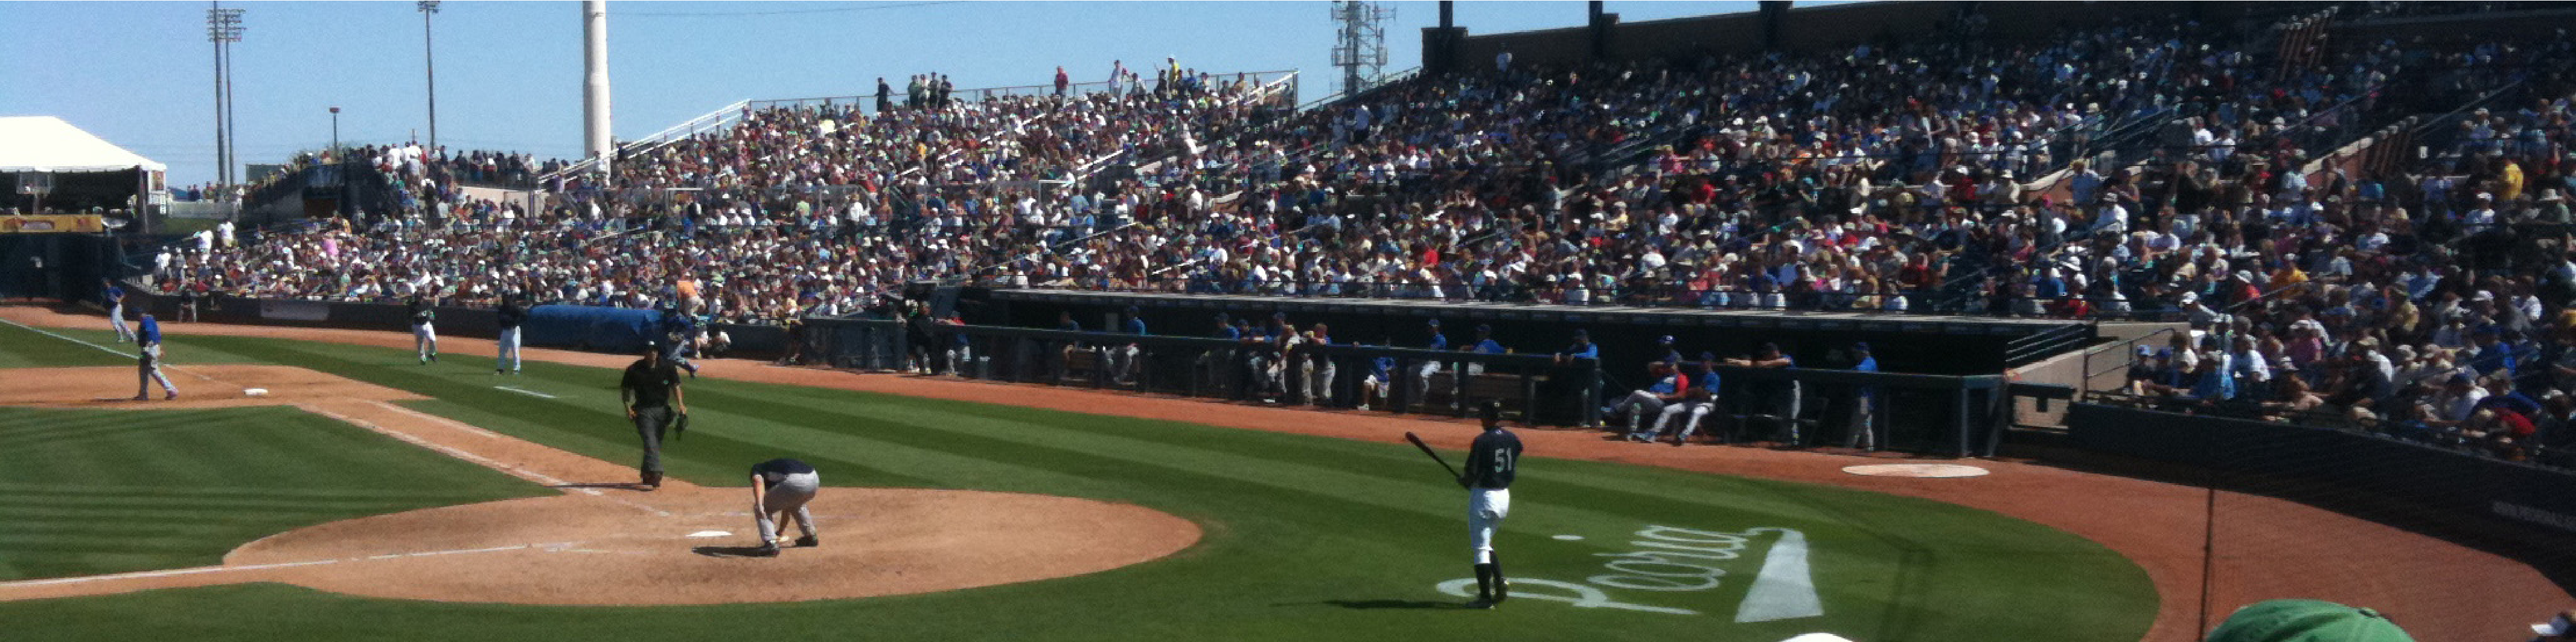
\includegraphics[width=\textwidth]{sampleteaser}
%  \caption{Seattle Mariners at Spring Training, 2010.}
%  \Description{Enjoying the baseball game from the third-base
%  seats. Ichiro Suzuki preparing to bat.}
%  \label{fig:teaser}
%\end{teaserfigure}

%\received{20 February 2007}
%\received[revised]{12 March 2009}
%\received[accepted]{5 June 2009}

%%
%% This command processes the author and affiliation and title
%% information and builds the first part of the formatted document.
\maketitle

\section{Introduction}
When a user of a geospatial information system (GIS) is searching for a specific location, they have many tools at their disposal. If they remember the exact name of the location they are looking for, most modern systems can return an exact match. If they know the physical address of the location, they can use that information to determine what they are looking for.

There are situations, however, where a user has access to imperfect information about a location they are searching for. Perhaps it is a location they visited a long time ago which has faded in memory or a vague recommendation from a friend. Perhaps they attempt to combine fragmented evidence for a police investigation or fuse intelligence in a military operation. 

Regardless of the reason, common approaches to the problem now see users employing GIS tools for their \textit{bold adjust} to get them to the correct general area and then rely on a manual \textit{last mile} effort typically involving the visual inspection of remote sensing imagery, searching for distinct landmarks or terrain features that match their partial information. The \textit{last mile} effort, while the most important, is also the bottleneck.

My proposed project asks \textit{is it possible to augment existing GIS systems with micro-terrain data, to elevate the bottleneck of the 'last mile' search}. 

\section{Outline of Work}
My project seeks to create a system that will allow a user to use micro-terrain features of a geographic location in their queries to replace the visual \textit{last mile} inspection. 

A production scale system would feature a number of components: 
\begin{enumerate}
    \item \textbf{Object Detection.} Object detection would be run over the source of the remote sensing imagery at the highest available resolution (i.e. closest to the ground). 
    \item \textbf{Feature Association.} Given a collection of locations and a collection of objects, determine which objects are associated with which feature. 
    \item \textbf{Concept Mapping.} Given a collection of locations and associated objects, develop concept maps to describe positional relationships of objects to each other and the location. 
    \item \textbf{Aggregation.} Given the mapped locations and objects, aggregate entities at different levels of resolution and update concept maps appropriately. 
    \item \textbf{Searching.} A query interface is minimally viable, but a mature system should support natural-language searching, reducing the burden on users.     
\end{enumerate}

All components less the searching would be pre-processed and stored. Given the scale of the work, external dependencies and scope of the class, I will focus my efforts on \textit{feature association}, \textit{concept mapping} and \textit{aggregation}. 

\section{Related Work}
There are several fields of related work, each at varying levels of maturity and utility for my project. 

Relevant to the \textbf{\textit{object detection}} component of my proposed system, 2018 efforts to improve the state of the art in object detection from remote sensing imagery focused on developing datasets for training and evaluating models. The xView project supports the detection of 60 classes of objects \cite{Lam2018} using horizontal bounding boxes. The DOTA project supports a much more modest 20 classes \cite{Xia2018}. Both focus towards shipping and industrial applications and so will not generalize well. The 2021 update to the DOTA project highlighted remote sensing object detection continues to suffer from issues of arbitrary rotation of objects and the vast disparities in the clustering of objects \cite{Ding2021}. DOTA version 2 tries to address these issues by employing \textit{orientation bounding boxes}, but is still very constrained in the classes of objects it supports. A separate effort by Li et. al in 2020 can detect objects less constrained to heavy industry but only accounts for 20 or so objects \cite{Li2020}. Overall current work on remote-sensing object detection indicates that it is still an emerging field that is incapable of supporting the labelling of micro-terrain features required for the proposed system, as a result, the object detection step is deliberately scoped out of my project. 

An area growing parallel with remote sensing object detection is that of \textit{image captioning and visual question answering}. In addition to implementing previously discussed object detection techniques, they employ alternate data sources to augment their ability to provide answers to natural language questions about remote sensing imagery. In 2017 Shi and Zhou demonstrated that it is possible to automate caption generation for remote sensing imagery, however, their experimentation showed it to be ineffective at tasks like counting objects \cite{Shi2017}, an important requirement of micro-terrain analysis. The paper that initiated the domain of Remote Sensing Visual Question Answering (RSVQA) was published in 2020 by Lobry et. al. and showed a good ability to answer direct questions about a given remote sensing image, including area estimates, object counts and determining the relative locations of objects. These capabilities are all useful in my \textit{\textbf{concept mapping}} component. Importantly they also incorporated geospatial information from OpenStreetMap into their system. A key limitation they identified is that the lack of information in OSM about specific micro-terrain features and the inability of object detection models to provide it presents a major gap holding back the advancement of the RSVQA field \cite{Lobry2020}. My work may contribute towards closing that gap. Later work by Zheng et. al. and Yuan et. al highlight that RSVQA is very much in its infancy, and they focus on improving the underlying models used in RSVQA systems \cite{Zheng2021, Yuan2022}. 

In addition to the gap identified by Lobry et. al, one of the limitations is the RSVQA approach is a focus on answering questions about the \textit{things that the user is already looking at}. In my partial-information use case, \textit{the user doesn't know exactly where to look}, so using the RSVQA approach would render no improvement to performance over the visual inspection itself. The real challenge is to identify \textit{where} to look, not \textit{what} they are looking at. 

Towards identifying where the user could be looking, the field of \textit{geospatial question answering}, related to \textit{geospatial information retrieval} offers promising directions. In 2018 Punjani et. al. sought to determine whether geospatial information could be incorporated into a question-answering system \cite{Punjani2018}. They used the established Frankenstein variant of the Qanary approach to developing question-answering pipelines to develop GeoQA. GeoQA can answer questions in several useful geospatial categories, including point queries, range queries and property-based queries. They built their system on linked data collected from OpenStreetMaps and WikiData. More recently, the efforts to develop WorldKG, a geospatial knowledge graph of the world extend the linked-data approach and allow users to generate SPARQL queries to answer complex geospatial questions across the fused knowledge of OpenStreetMaps, DBPedia and WikiData \cite{Dsouza2021}. These linked data approaches to geospatial question answering are valuable advancements but do not include enough micro-terrain detail to satisfy the requirement of my project to allow a user to find a location based on partial information about the micro-terrain of the location. 

\textbf{Geospatial clustering.} I could not locate any work specific to assigning membership of objects to class based on geospatial proximity. However, given the nature of the task where proximity is a strong indicator of ownership, it seems likely that a naive approach employing nearest neighbour or another clustering approach where the centroids of the clusters are the 'parent' locations will be sufficient. 

\section{Plan and Timeline}
\begin{itemize}
    \item \textbf{14 Mar.} Submit Project Proposal
    \item \textbf{26 Mar.} 3 x Object Labeled areas generated. 
    \item \textbf{02 Apr.} Location retrieval from OSM implemented.
    \item \textbf{09 Apr.} Ownership Clustering Implemented.
    \item \textbf{16 Apr.} Concept Mapping Implemented.
    \item \textbf{23 Apr.} Proof-of-concept querying implemented. 
    \item \textbf{30 Apr.} Draft Paper Complete
    \item \textbf{04 May.} \textit{Assumed} Deadline for submission
    \item \textbf{11 May.} \textit{Assumed} Class Presentation
\end{itemize}

\section{Conclusion}
My project proposes to help users with incomplete information about a location use micro-terrain features to identify the location they are searching for. It aims to leverage recent advances in geospatial and remote-sensing visual question-answering to enhance the existing work on identifying locations at the macro level. 

%%
%% The next two lines define the bibliography style to be used, and
%% the bibliography file.
\bibliographystyle{ACM-Reference-Format}
\bibliography{sample-base, CSMC828T_project}

%%
%% If your work has an appendix, this is the place to put it.
\appendix

\end{document}
\endinput
%%
%% End of file `sample-authordraft.tex'.
